\documentclass{standalone}

\usepackage{tikz}
\usetikzlibrary{shapes.geometric, arrows}

\tikzstyle{stylein} = [rectangle, rounded corners, minimum width=1.1cm, minimum height=1cm,text centered, draw=black, fill=red!30]

\tikzstyle{styleout} = [rectangle, rounded corners, minimum width=1.1cm, minimum height=1cm,text centered, draw=black, fill=blue!30]

\begin{document}
	
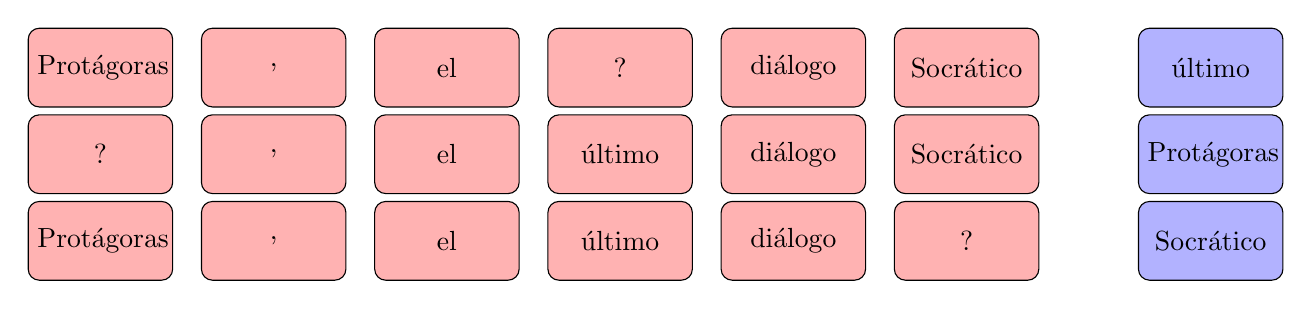
\begin{tikzpicture}[node distance=1.1cm]
\node (f41) [stylein, text width=1.6cm] {Protágoras};
\node (f42) [stylein, text width=1.6cm, right of=f41, xshift=1.1cm] {,};
\node (f43) [stylein, text width=1.6cm, right of=f42, xshift=1.1cm] {el};
\node (f44) [stylein, text width=1.6cm, right of=f43, xshift=1.1cm] {?};
\node (f45) [stylein, text width=1.6cm, right of=f44, xshift=1.1cm] {diálogo};
\node (f46) [stylein, text width=1.6cm, right of=f45, xshift=1.1cm] {Socrático};
\node (o4) [styleout, text width=1.6cm, right of=f46, xshift=2cm] {último};

\node (f51) [stylein, text width=1.6cm, below of=f41] {?};
\node (f52) [stylein, text width=1.6cm, right of=f51, xshift=1.1cm] {,};
\node (f53) [stylein, text width=1.6cm, right of=f52, xshift=1.1cm] {el};
\node (f54) [stylein, text width=1.6cm, right of=f53, xshift=1.1cm] {último};
\node (f55) [stylein, text width=1.6cm, right of=f54, xshift=1.1cm] {diálogo};
\node (f56) [stylein, text width=1.6cm, right of=f55, xshift=1.1cm] {Socrático};
\node (o5) [styleout, text width=1.6cm, right of=f56, xshift=2cm] {Protágoras};

\node (f61) [stylein, text width=1.6cm, below of=f51] {Protágoras};
\node (f62) [stylein, text width=1.6cm, right of=f61, xshift=1.1cm] {,};
\node (f63) [stylein, text width=1.6cm, right of=f62, xshift=1.1cm] {el};
\node (f64) [stylein, text width=1.6cm, right of=f63, xshift=1.1cm] {último};
\node (f65) [stylein, text width=1.6cm, right of=f64, xshift=1.1cm] {diálogo};
\node (f66) [stylein, text width=1.6cm, right of=f65, xshift=1.1cm] {?};
\node (o6) [styleout, text width=1.6cm, right of=f66, xshift=2cm] {Socrático};

\end{tikzpicture}

\end{document}